\graphicspath{{images/}}

\begin{appendices}
  \section{Random Forest Models}

  \subsection{Bootstrapping} \label{app:sec:bootstrapping}

  Random Forest Models are made powerful as a result of the randomness injected into each tree by the boostrapping process.
  Each individual decision tree is constructed on a \textbf{bootstrapped} subset of the available data: that is, if we have a dataset containing $n$ observations,
  \textbf{bootstrapping is the process of sampling $n$ instances with replacement}.

  Further, if we have a dataset containing $p$ features, bootstrapping can also be used to randomly select a subset of the available features to be used in the tree-building process, which allows the random forest model to be less susceptible to overfitting.

  In practice, this means that some instances in the available data will be selected more than once whereas some instances won't be selected at all. In fact, the probability of an instance being dropped entirely due to bootstrapping is given by $ (1- \frac{1}{n})^n$, the value of which can be proven to be equal to approximately $\frac{1}{3}$.
  \textbf{This implies that a third of the instances in the original data will be left out in each tree when bootstrapping n samples with replacement.}

  One of the biggest positives resulting from the bootstrapping process is that considering the fact that each tree only uses two-thirds of the available data, trees generated in the random forest models usually differ significantly from each other.

  The bootstrapping process gives us a good metric to judge the performance of a Random Forest model, namely the \textbf{Out of Bag Error} (more commonly shortened as OOB Error).
  As mentioned before, about a third of the instances in the original data are not selected for the tree-building process.
  After building a tree with the $n$ bootstrapped observations, one can test the model against each of the instances in the third of observations that were left out, and calculate the average prediction error from those samples. The overall out of bag error for the model can subsequently be calculated by averaging the OOB score for each tree generated by the random forest model.

  \subsection{Bagging} \label{app:sec:bagging}

  Bagging is the process of growing a tree where each node in the tree looks at every value in the boostrapped sample in every feature to find the best split in the data at that particular node. This process is then repeated for every single tree generated in the random forest model.

  Random Forests incorporate bagging with a subtle difference: While bagging considers every feature to find the best split in the data at a given node, each tree in a Random Forest model only looks at a subset of the available features.
  As opposed to using the same set of features in every single tree, choosing a subset of the available features helps inject more randomness into the model thereby making it less susceptible to overfitting whilst experimenting with interactions between varying sets of features.

  \section{Implementation Detail}

  \subsection{Decision Tree Implementation} \label{app:sec:dt_implementation}

  \textbf{The implementation of this classifier can be found in the \textit{DecisionTreeClassifier.py} file attached along with this submission.}

  The implementation of the custom implementation of the decision tree classifier was implemented in the \textbf{Object-Oriented} (OO) paradigm using \textbf{Python}.

  A Decision Tree Classifier object created using the implementation has the following parameters:
  \begin{itemize}
    \item \texttt{max\_depth}: This refers to the maximum depth of the tree. If set to None, the tree will grow until all leaves are pure, or until it reaches the minimum samples split.
    \item \texttt{min\_samples\_split}: The minimum number of samples required to split an internal node or branch.
    \item \texttt{max\_features}: The number of features to be considered when looking for the optimal split. If None, all features are considered.
    \item \texttt{min\_impurity\_decrease}: A node will be split if this split induces a decline in impurity that is greater than or equal to this value.
    \item \texttt{random\_state}: Controls the randomness of the bootstrapping in the samples used when the trees are built.
    \item \texttt{debug}: Flag to set the logging information specificity.
  \end{itemize}

  The \textbf{attribute(s)} associated with the object include:
  \begin{itemize}
    \item \texttt{root} (Node): Root node of the decision tree post-fitting.
  \end{itemize}

  The \textbf{methods} applicable to the object include:
  \begin{itemize}
    \item \texttt{fit(X,y)}: Fits the decision tree model to the given dataset.
    \item \texttt{predict (X)}: Predicts the class labels for the given dataset.
    \item \texttt{visualize\_tree(feature\_names, class\_names)}: Generates an image of the decision tree using the \textit{graphviz} library.
  \end{itemize}

  Technical specification of the classifier's parameters are summarized in ~\autoref{tab:dt_parameters}.

  \begin{table}[H]
    \centering
    \begin{tabular}{lccc}
      \toprule
      \textbf{Parameter}      & \textbf{Data Type} & \textbf{Optional?} & \textbf{Default Value} \\
      \midrule
      max\_depth              & int                & yes                & None                   \\
      min\_samples            & int                & yes                & 2                      \\
      max\_features           & int                & yes                & None                   \\
      min\_impurity\_decrease & float              & no                 & 0                      \\
      random\_state           & int                & yes                & 42                     \\
      debug                   & bool               & yes                & FALSE                  \\
      \bottomrule
    \end{tabular}
    \caption{DT - Parameter Settings}
    \label{tab:dt_parameters}
  \end{table}

  \subsubsection{Pseudocode: How it Works}

  In general, decision trees are synthesized using the training data available. The decision tree algorithm recursively builds the tree \cite{bhiksha} by:
  \begin{itemize}
      \item Step 1: All available observations in the training dataset are assigned to the root node of the tree. The current node is then set to the root node.
      \item Step 2: For every single feature available, training data instances are separated by their values for the associated feature. The information gain is then calculated for this separation or partition.
      \item Step 3: The current node is then set to be the feature which resulted in the greatest information gain in the previous step. When the optimal information gain is equal to 0, that node can be considered to be a leaf node.
      \item Step 4: Repeat the separation process according to the value of the best feature, just as in step two of this algorithm described above.
      \item Step 5: Mark every layer of separation to be a child node to the current node.
      \item Step 6: If a child node contains only instances from a singular class, then mark it as a leaf, and return. If not, set the current node to be this child note and repeat from step two recursively until all options are exhausted.
  \end{itemize}

    A generalized flowchart of such a decision tree classifier is shown in ~\autoref{fig:dt_flowchart}:

    \begin{figure}[H]
    \centering
    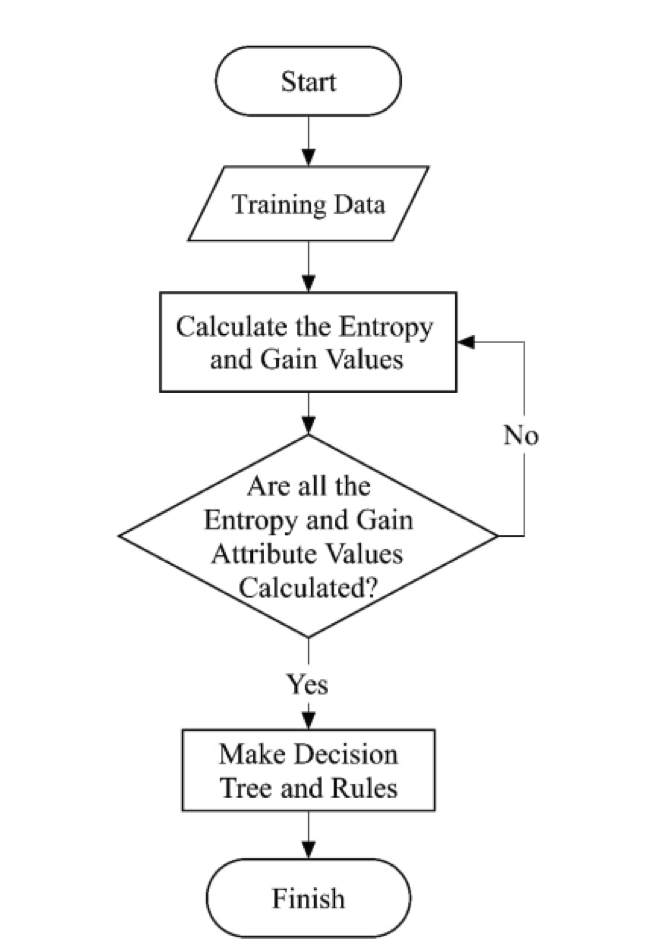
\includegraphics[width=0.65\textwidth]{images/id3-dt.png}
    \caption{Training a Decision Tree}
    \label{fig:dt_flowchart}
    \end{figure}
    \FloatBarrier


  \subsection{Random Forest Classification Implementation} \label{app:sec:rf_implementation}

  \textbf{The implementation of this classifier can be found in the \textit{RandomForestClassifier.py} file attached along with this submission.}

  Similar to the implementation of the Decision Tree Classifier, the Random Forest Classifier was also implemented using the OO paradigm in Python. The class builds a specified number of decision trees, each of which is trained on a bootstrapped sample of the input data.
  \textbf{For predictions, it aggregates the predictions of all trees using majority voting}.
  In addition, it also calculates the Out-Of-Bag score as an additional metric to estimate model performance.

  The Random Forest Classifier has the same hyperparameters as the Decision Tree Classifier considering they both involve controlling how much a tree can grow. In addition, it also has the hyperparameters seen in a typical bagging classifier to control the ensemble of trees in itself:
  \begin{itemize}
    \item \texttt{n\_estimators}: The number of trees in the forest.
    \item \texttt{max\_depth}: This refers to the maximum depth of the tree. If set to None, the tree will grow until all leaves are pure, or until it reaches the minimum samples split.
    \item \texttt{min\_samples\_split}: The minimum number of samples required to split an internal node or branch.
    \item \texttt{max\_features}: The number of features to be considered when looking for the optimal split. If None, all features are considered.
    \item \texttt{min\_impurity\_decrease}: A node will be split if this split induces a decline in impurity that is greater than or equal to this value.
    \item \texttt{random\_state}: Controls the randomness of the bootstrapping in the samples used when the trees are built.
    \item \texttt{debug}: Flag to set the logging information specificity.
  \end{itemize}

  The \textbf{attribute(s)} associated with the object include:
  \begin{itemize}
    \item \texttt{oob\_score}: A floating point value, referring to the model's performance on unseen data.
    \item \texttt{trees} : A list of DecisionTreeClassifier objects to represent the list of fitted decision tees within the forest.
  \end{itemize}

  The \textbf{methods} applicable to the object include:
  \begin{itemize}
    \item \texttt{fit(X,y)}: Fits the Random Forest Classifier to the given dataset.
    \item \texttt{predict (X)}: Predicts the class labels for the given dataset.
    \item \texttt{\_bootstrap\_sample(X, y)}: Generates a bootstrapped sample from the input dataset and identifies OOB indices.
    \item \texttt{\_calculate\_oob\_score(oob\_votes, y)}: Calculates the OOB score based on the aggregated OOB predictions.
  \end{itemize}

  Technical specifics of the classifier's parameters are summarized in ~\autoref{tab:rf_parameters}.

  \begin{table}[H]
    \centering
    \begin{tabular}{lccc}
      \toprule
      \textbf{Parameter}      & \textbf{Data Type} & \textbf{Optional?} & \textbf{Default Value} \\
      \midrule
      n\_estimators           & int                & yes                & 100                    \\
      max\_depth              & int                & yes                & None                   \\
      min\_samples            & int                & yes                & 2                      \\
      max\_features           & int                & yes                & None                   \\
      min\_impurity\_decrease & float              & no                 & 0                      \\
      random\_state           & int                & yes                & 42                     \\
      debug                   & bool               & yes                & FALSE                  \\
      n\_jobs                 & int                & yes                & -1                     \\
      verbose                 & int                & yes                & 10                     \\
      \bottomrule
    \end{tabular}
    \caption{RF - Parameter Settings}
    \label{tab:rf_parameters}
  \end{table}

    \subsubsection{Pseudocode: How it Works}

    As discussed before, the Random Forest model is an ensemble learning method that combines the output of many decision trees to get a single result, using the processes of bagging and bootstrapping. 
  In general, Random Forests are synthesized using multiple decision trees constructed from randomly selected subsets of the training data. The Random Forest algorithm builds these trees and aggregates their predictions by \cite{bernstein}:

    \begin{itemize}
        \item Step 1: For each tree in the Random Forest:
        \begin{itemize}
            \item Step 1.1: Randomly select a subset of the training data with replacement (bootstrapping).
            \item Step 1.2: Build a decision tree using the selected subset:
            \begin{itemize}
                \item Step 1.2.1: Assign all observations in the subset to the root node of the tree.
                \item Step 1.2.2: For a randomly selected subset of features, calculate the information gain for each feature.
                \item Step 1.2.3: Choose the feature with the highest information gain as the current node.
                \item Step 1.2.4: Repeat the separation process according to the value of the best feature.
                \item Step 1.2.5: Mark each layer of separation as a child node to the current node.
                \item Step 1.2.6: If a child node contains only instances from a single class, mark it as a leaf. Otherwise, set the current node to this child node and repeat from Step 1.2.2.
            \end{itemize}
        \end{itemize}
        \item Step 2: For each new observation, make a prediction by aggregating the predictions from all the trees in the Random Forest (e.g., majority vote for classification or averaging for regression).
    \end{itemize}

    This is summarized visually in ~\autoref{fig:rf_flowchart}:
    
    \begin{figure}[H]
      \centering
      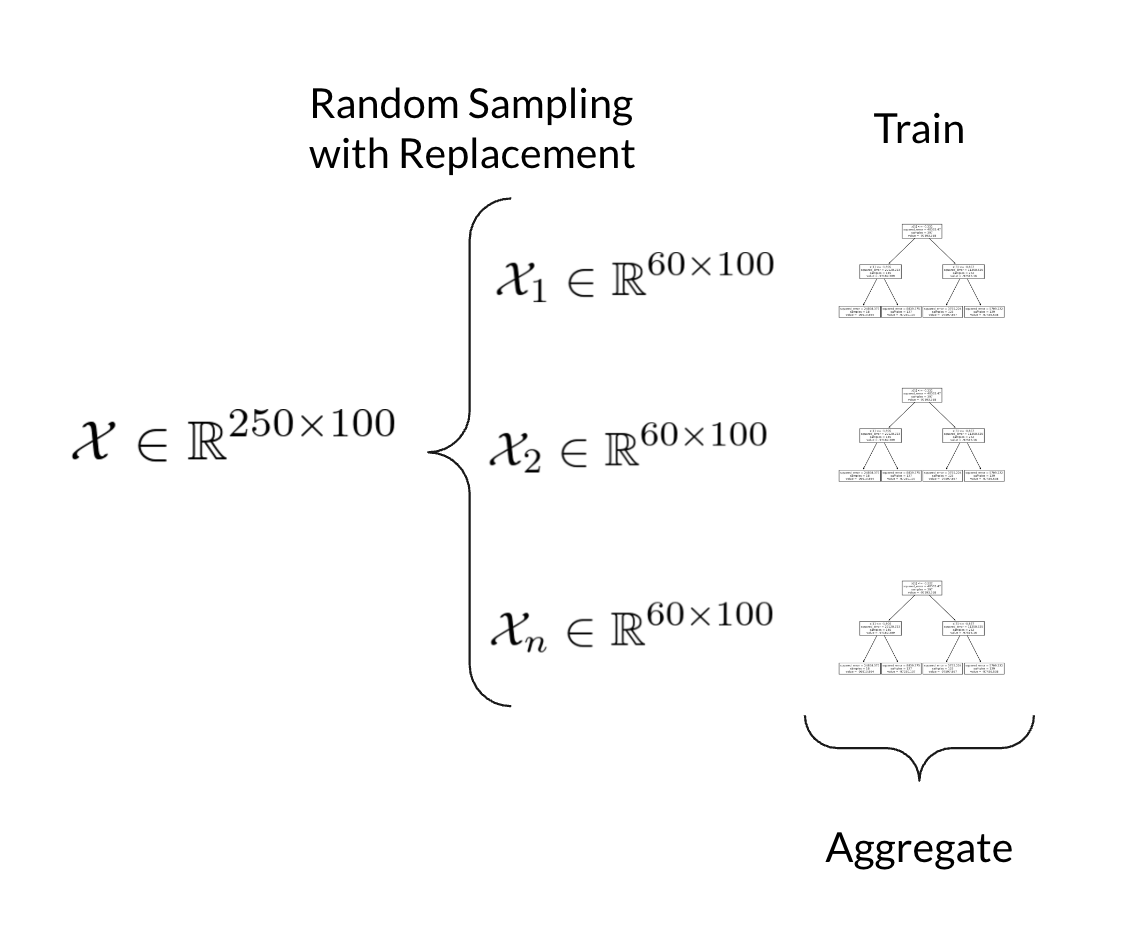
\includegraphics[width=0.65\textwidth]{images/rf_train.png}
      \caption[Illustration of training a Random Forest Model.]{Illustration of training a Random Forest Model.\protect \footnotemark}
      \label{fig:rf_flowchart}
    \end{figure}
    \footnotetext{Source: \href{https://en.wikipedia.org/wiki/Random_forest}{Wikipedia}}
    \FloatBarrier
    
    \subsection{Gradient Boosting Classification Implementation} \label{app:sec:gb_implementation}
    
  \textbf{The implementation of this classifier can be found in the \textit{GradientBoostingClassifier.py} file attached along with this submission.}

  Adhering to the Object-Oriented (OO) paradigm in Python, this classifier is constructed to address binary classification tasks through an ensemble of decision trees.

  The class GradientBoostingClassifier is equipped with the following parameters:
  \begin{itemize}
    \item \texttt{n\_estimators}: The number of trees to build. Default is 100.
    \item \texttt{learning\_rate}: The learning rate controls the contribution of each tree. Default is 0.1.
    \item \texttt{max\_depth} (optional): The maximum depth of each tree. If None, the trees will grow until all leaves are pure.
    \item \texttt{min\_samples\_split}: The minimum number of samples required to split an internal node. Default is 2.
    \item \texttt{max\_features} (optional): The number of features to consider when looking for the best split. If None, all features are considered.
    \item \texttt{min\_impurity\_decrease}: A node will be split if this split induces a decrease of the impurity greater than or equal to this value. Default is 0.0.
    \item \texttt{random\_state} (optional): Controls the randomness of the bootstrapping of the samples used when building trees. Default is None.
    \item \texttt{debug}: If True, the logging level will be set to DEBUG, providing more detailed logging information. Default is False.
  \end{itemize}

  The \textbf{attribute(s)} associated with the object include:
  \begin{itemize}
    \item \texttt{trees} (List[DecisionTreeClassifier]): The list of fitted trees.
    \item \texttt{f0} (float): The initial prediction of the model.
  \end{itemize}

  The \textbf{methods} applicable to the object include:
  \begin{itemize}
    \item \texttt{fit(X, y)}: Fits the gradient boosting model to the given dataset.
    \item \texttt{predict(X)}: Predicts the class labels for the given dataset.
  \end{itemize}

  Additionally, the \texttt{sigmoid}, \texttt{log\_loss}, and gradient methods handle the mathematical computations necessary for the model's training process.

  Technical specifics of the classifier's parameters are summarized in ~\autoref{tab:gb_parameters}.

  \begin{table}[H]
    \centering
    \begin{tabular}{lccc}
      \toprule
      \textbf{Parameter}      & \textbf{Data Type} & \textbf{Optional?} & \textbf{Default Value} \\
      \midrule
      n\_estimators           & int                & yes                & 100                    \\
      learning\_rate          & float              & no                 & 0.1                    \\
      max\_depth              & int                & yes                & None                   \\
      min\_samples\_split     & int                & no                 & 2                      \\
      max\_features           & int                & yes                & None                   \\
      min\_impurity\_decrease & float              & no                 & 0.0                    \\
      random\_state           & int                & yes                & None                   \\
      debug                   & bool               & yes                & False                  \\
      \bottomrule
    \end{tabular}
    \caption{GB Parameter Settings}
    \label{tab:gb_parameters}
  \end{table}
\end{appendices}
